%SourceDoc ../YourName-Dissertation.tex
\vspace*{-80mm}
\chapter{Conservation Equations} \label{chapter2:conservation_equations}
	
	
\section{Single Phase Liquid Euler Equations} \label{sec:euler_equations}
	
	The finite volume structure in COBRA-TF in figure \ref{fig:CTF-Cells} is for
	a one-dimmensional channel in the axial direction with $n$ number of cells.
	The first and last cells at $0$ and $n+1$ are ghost cells and act as the
	boundary conditions for the problem. Pressure, enthalpy, and density are
	averaged over the cell volume and are located at the center of the cell.
	Mass flow rate and velocity are located at the faces in between cells. The
	cells are represented with an index $i$, and the faces with indexes of
	$i+\frac{1}{2}$ or $i-\frac{1}{2}$. This project will initially focus
	on this 1-D configuration. Usually the code is three dimensional, with
	channels connecting to each other in two more dimmensions. Fully 3-D
	equations will be considered in future work.
	
	\begin{figure}[!h]
		\centering
		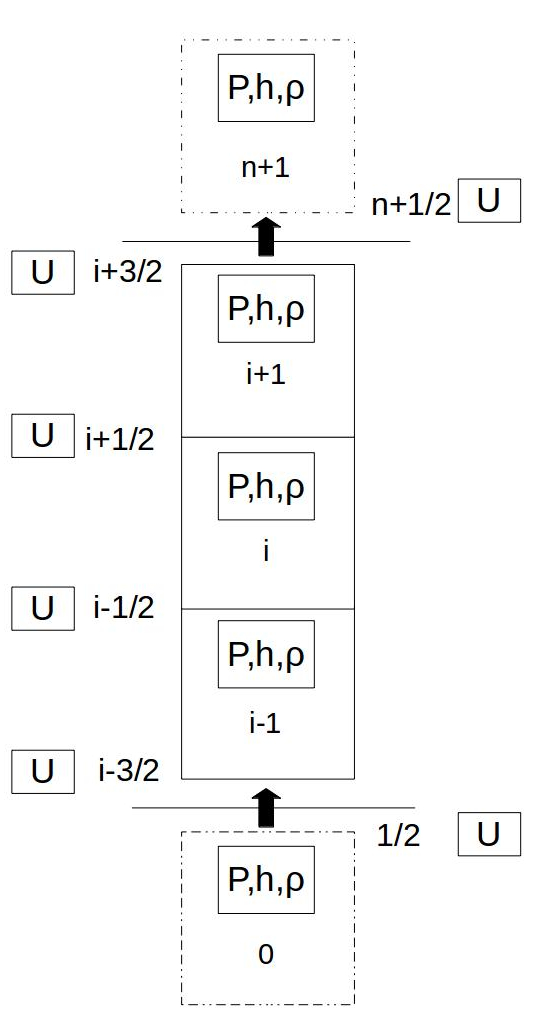
\includegraphics[width=0.30\textwidth]{images/CTF-Cells}
		\caption{The finite volume structure for COBRA-TF}
		\label{fig:CTF-Cells}
	\end{figure}

	The thermal hydraulics of a LWR core is an important part of nuclear
	reactor desigin. COBRA-TF solves 8 conservation equations for liquid,
	entrained droplet, and vapor phases of water boiling within the rod structure
	of a LWR reactor core \cite{Salko2014}. Currently, the conservation
	equations analytically reduce into a pressure matrix in a semi-implicit
	method with rod temperatures solved for explicitly. This work involves
	representing the 1-D single phase liquid conservation equations and calculated 
	variables in a residual formulation. The full jacobian matrix can then be
	built numerically, and  can then either be reduced to a pressure matrix or
	solved directly. Verification of the residuals was done by comparing
	calculated results to analytical solutions for isokinetic advection and shock
	tube problems. For each verification problem, a scaling study of the
	truncation error was compared to the predicted behaviour derived from modified
	equation analysis using Richardson extrapolation. Further work was then
	applied to represent 1-D heat conduction within the heater rods. Some initial
	work was done to allow the code to solve either semi-implicitly, or fully impicitly.
    The single phase Euler partial differential equations for mass
    \eqref{eq:pde_mass}, momentum \eqref{eq:pde_momentum}, and energy
    \eqref{eq:pde_energy} corresond to the unknown variables density $\rho$,
    velocity $u$, pressure $P$, and enthalpy $h$. The first terms in each of the
    equations are temporal terms. The rest of the terms are steady state spatial
    terms. The last term in the energy equation represents the net heat transfer
    from the adjacent rods to the current fluid subchannel.
    
    \begin{equation}
    	\label{eq:pde_mass}
    	\frac{ \partial \rho}{\partial t} + \bigtriangledown \rho u = 0
    \end{equation}
    
    \begin{equation}
    	\label{eq:pde_momentum}
    	\frac{ \partial \rho u}{\partial t} + \bigtriangledown \rho u^{2} +
    	\bigtriangledown P - \rho g  = 0
    \end{equation}
    
    \begin{equation}
    	\label{eq:pde_energy}
    	\frac{ \partial \rho h}{\partial t} -
    	\frac{ \partial  P}{\partial t} + 
    	\bigtriangledown ( \rho  u h )%  -
    	+ \frac{q_{rod}}{\forall_{fluid}}
    	%u \frac{ \partial  P}{\partial x}
    	= 0
    \end{equation}
    
    The 1-D formulation of the Euler Equations will assume a direction $x$ as shown
    in the 1-D mass equation \eqref{eq:1-D_mass}. The momentum and energy equations
    are represented in a non-conservative form as shown in equations
    \eqref{eq:1-D_momentum_long} and \eqref{eq:1-D_energy_long}. The momentum
    equation contains a term that has a product of the left hand side of the 1-D
    mass equation. This terms can therefore be dropped since it is equivalent
    to zero, and the entire equation can be divided by density to give a simpler
    form of the momentum equation \eqref{eq:1-D_momentum}. The last term in the
    energy equation represents the net heat transfer from the adjacent rods to
    the current fluid subchannel. This is equated as the surface area of
    the rod liquid interface times the heat transfer coefficient and temperature
    difference between the wall and bulk fluid temperatures. 
    
    \begin{equation}
    	\label{eq:1-D_mass}
    	\dfrac{ \partial \rho }{ \partial t} +
    	\dfrac{ \partial \rho u}{\partial x} = 0
    \end{equation}
    
    \begin{equation}
    	\label{eq:1-D_momentum_long}
    	\rho \dfrac{ \partial u }{ \partial t } + 
    	u \left(  \dfrac{ \partial \rho }{ \partial t } +
    	          \dfrac{ \partial \rho u }{\partial x} \right) +
    	\rho u \dfrac{ \partial u}{ \partial x} + 
    	\dfrac{ \partial P}{ \partial x}   - \rho g
    	= 0
    \end{equation}
    
    \begin{equation}
    	\label{eq:1-D_momentum}
    	\dfrac{ \partial u }{ \partial t } + 
    	u \dfrac{ \partial u }{ \partial x } + 
    	\dfrac{1}{ \rho } \dfrac{ \partial P }{ \partial x } - g  
    	= 0
    \end{equation}
    
    \begin{equation}
    	\label{eq:1-D_energy_long}
    	\rho \frac{ \partial  h}{\partial t} -
    	     \frac{ \partial  P}{\partial t} + 
    	h    \frac{ \partial  \rho}{\partial t} +
    	\rho u \frac{ \partial h }{ \partial x} +
    	h    \frac{ \partial \rho u }{ \partial x} 
    	+ \frac{2\pi r_{rod}}{A_{i}}h_{l}\left(T_{wall}-T_{fluid}\right)
    	= 0
    \end{equation}
    
    The 1-D equations are then evaluated at a position index $ i $ and a certian time
    $n$ in order to solve for the next time value of $n+1$. In the mass equation
    \eqref{eq:FD_mass}, the velocities are located at the cell faces
    $i+\frac{1}{2}$ and $i-\frac{1}{2}$. The density at a corresponding face is
    either upwinded $\dot{\rho}_{i+\frac{1}{2}}^{n}$, or averaged
    $\bar{\rho}_{i+\frac{1}{2}}^{n}$. In equation \eqref{eq:FD_momentum}, the
    derivative $\frac{ \partial u}{ \partial x}$ is upwinded assuming that the
    flow is positive. In the energy equation, \eqref{eq:FD_energy} the enthalpy
    values in the first spatial term are upwinded and shown here assuming a
    positive velocity. The equation of state \eqref{eq:EOS} solves for density
    assuming that it is a linear combination of changes due to pressure and
    enthalpy. The partial derivatives in the equation are calculated from
    steam tables as functions of old time pressure and enthalpy. 
    
    \begin{equation}
    	\label{eq:FD_mass}
    	\frac{ \rho_{i}^{n+1}-\rho_{i}^{n}}{ \Delta t} +
    	\frac{ \dot{\rho}_{i+\frac{1}{2}}^{n} u_{i+\frac{1}{2}}^{n+1}  -
    	\dot{\rho}_{i-\frac{1}{2}}^{n}  u_{i-\frac{1}{2}}^{n+1} }{\Delta x}
    	 = 0
    \end{equation}
    
    \begin{equation}
    	\label{eq:FD_momentum}
    	\frac{  u_{i+\frac{1}{2}}^{n+1} - u_{i+\frac{1}{2}}^{n} }{ \Delta t } + 
    	u_{i+\frac{1}{2}}^{n} \left( \frac{  u_{i+\frac{1}{2}}^{n} -
    	u_{i-\frac{1}{2}}^{n}}{ \Delta x} \right) +
    	\frac{1}{\bar{\rho}_{i+\frac{1}{2}}^{n} } 
    	\frac{ P_{i+1}^{n+1} -P_{i}^{n+1} }{ \Delta x } - g
    	= 0
    \end{equation}
    
    \begin{multline}
    	\label{eq:FD_energy}
    	\rho_{i}^{n} \frac{ h_{i}^{n+1} - h_{i}^{n}}{\Delta t} 
    	+ h_{i}^{n} \frac{ \rho_{i}^{n+1} - \rho_{i}^{n}}{\Delta t} 
    	- \frac{P_{i}^{n+1}-P_{i}^{n}}{\Delta t}
    	+ \left( \rho u \right)_{i}^{n} 
    		\frac{   h _{i}^{n}  - h _{i-1}^{n} }{\Delta x}  \\
    	+ h _{i}^{n} \frac{ \dot{\rho}_{i+\frac{1}{2}}^{n} u_{i+\frac{1}{2}}^{n+1} 
    	- \dot{\rho}_{i-\frac{1}{2}}^{n}  u_{i-\frac{1}{2}}^{n+1} }{\Delta x}
    	+ \frac{2\pi r_{rod}}{A_{i}}h_{l}\left(T_{wall}-T_{fluid}\right)
    	= 0
    \end{multline}
    
    \begin{equation}
    	\label{eq:EOS}
    	\rho_{i}^{n+1} - \rho_{i}^{n} = 
    	\left( \frac{ \partial \rho }{\partial P} \right) 
    	\left( P_{i}^{n+1} - P_{i}^{n} \right)
    	+ 
    	\left( \frac{ \partial \rho }{\partial h} \right) 
    	\left( h_{i}^{n+1} - h_{i}^{n} \right)
    \end{equation}

\section{1-D Radial Solid Conduction Equation} \label{sec:rad_conduction}

The conduction equation for a cylindrical system is given in equation \ref{eq:full_conduction}.
The first  term represents the amount of energy stored within the solid area within
a unit  time. The second term is the conduction in the radial direction. The
second  and third terms are the conduction in the azimuthal and axial
directions,  respectively. The last term represents the heat generation within
the solid.

\begin{equation}
	\label{eq:full_conduction}
	  \rho_{i}c_{p,i}\frac{\partial T}{\partial t}
	- \frac{1}{r}\frac{\partial}{\partial r}\left( 
		kr\frac{\partial T}{\partial r}\right)
	- \frac{1}{r^{2}}\frac{\partial}{\partial \theta}\left(
		k\frac{\partial T}{\partial \theta}\right)
	- \frac{\partial}{\partial z}\left(k\frac{\partial T}{\partial z}\right) 
	- q'''
	= 0
\end{equation}

This work focuses on the 1D radial equations setting the derivatives with
respect to the angular and axial directions to zero. Equation \ref{eq:full_conduction} now reduces
to equation \ref{eq:rad_conduction}.

\begin{equation}
	\label{eq:rad_conduction}
	  \rho_{i}c_{p,i}\frac{\partial T}{\partial t}
	- \frac{1}{r}\frac{\partial}{\partial r}\left( 
		kr\frac{\partial T}{\partial r}\right)
	- q'''
	= 0
\end{equation}

When the radius is zero, the fuel temperature is considered to be a maximum
giving the boundary condition in equation \ref{eq:bc_centerline}

\begin{equation}
	\label{eq:bc_centerline}
	\left(\frac{\partial T}{\partial r}\right)_{r=0}=0
\end{equation}

\begin{figure}[!h]
	\centering
	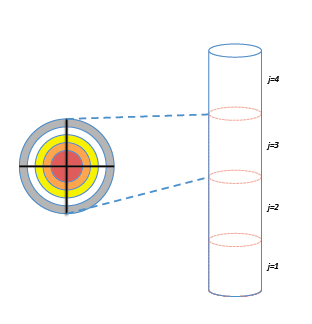
\includegraphics[width=0.40\textwidth]{images/rod-axial.png}
	\caption{Rod Axial}
	\label{fig:rod-axial}
\end{figure}

The nuclear rod geometry types in CTF are meshed at each axial level according
to figure \ref{fig:rod-axial}. Each axial level will be meshed as seen in figure
\ref{fig:radial_diagram} where the red region is fuel and the grey region is
cladding. The black dots represent the nodes within the fuel. Each node covers
a region within the rod as bounded by the dashed lines. The nodes within the
fuel are located at the center of the region. Each region is assumed to have
uniform properties with values evaluated at the node. The last node within  the
fuel is located at the surface of the fuel at the interface with the gap. 
There are two additional nodes that represent the outer clad surface and the
inner  clad surface respectively. The gap between the outer surface of the fuel
and the inner surface of the cladding has a specified heat transfer coefficient
or is calculated using the dynamic gap conductance model.

	\begin{figure}[!h]
		\centering
		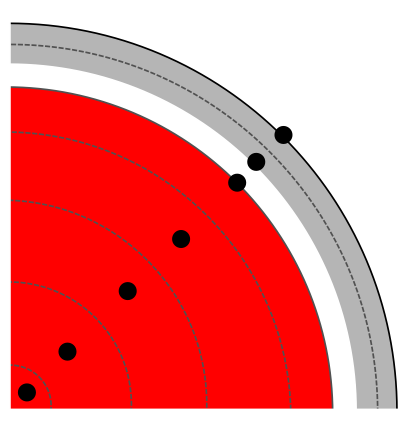
\includegraphics[width=0.40\textwidth]{images/radial_diagram.png}
		\caption{Radial Rod Meshing}
		\label{fig:radial_diagram}
	\end{figure}
	
The outer surface of the cladding is assumed to be in contact with the fluid in
the  adjacent channel on that axial level. The rods have the same number of
axial  levels as the fluid, but do not have ghost cells at the top and bottom.
Instead  the first and last fluid axial levels are connected to two rod axial
levels as  shown by Figure \ref{fig:fluid-solid-meshing}, where the rod axial
levels are on the left, and the fluid  axial levels are on the right. The light
blue cells are the fluid ghost cells.

	\begin{figure}[!h]
		\centering
		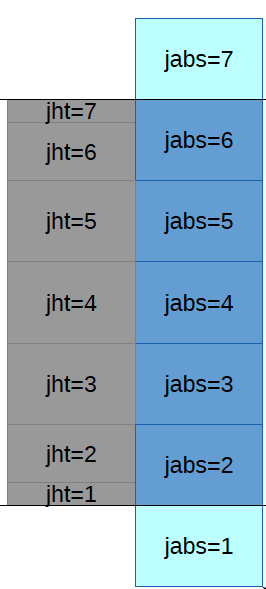
\includegraphics[width=0.20\textwidth]{images/fluid-solid-meshing.png}
		\caption{Radial Rod Meshing}
		\label{fig:fluid-solid-meshing}
	\end{figure}

The conduction equation can be approximated using the finite difference method,
or the control volume difference method \cite{Botte2000}. The control volume
method will be used  since it is the same method utilized in the original
version of CTF. The implicit  finite difference equation now looks like equation
\ref{eq:rod:fuel:conduction}.

\begin{equation}
	\small
	\label{eq:rod:fuel:conduction}
	  \rho_{i}c_{p,i}\frac{T^{n+1}_{i}-T^{n}_{i}}{\Delta t}
	- \frac{2\pi}{A_{i}}\left( 
		\left(k_{i+\frac{1}{2}}r_{i+\frac{1}{2}}
		\frac{T^{n+1}_{i+1}-T^{n+1}_{i}}{\Delta r_{i+\frac{1}{2}}}\right)
 	  - \left(k_{i-\frac{1}{2}}r_{i-\frac{1}{2}}
		\frac{T^{n+1}_{i}-T^{n+1}_{i-1}}{\Delta r_{i-\frac{1}{2}}}\right)
	  \right)
	- q_{i}'''
	= 0
\end{equation}

The density on the temporal term is defined as the cold mass of the node divided
by the current volume of the node, so that mass is not lost in the presence of
expansion. The temporal derivative is approximated with first order accurate
forward differencing. The spatial derivatives are evaluated at the right
boundary, $i+\frac{1}{2}$, and at the left boundary,$i-\frac{1}{2}$ using first
order forward differencing. When $i=1$ at the inner most node, the radius at the
left boundary and the derivative of the temperature is zero. At the boundary
between the surface of the fuel and the inside surface of the cladding, a
different set of finite difference equations are needed as given by equation
\ref{eq:rod:fuel_surface:conduction}

\begin{equation}
	\label{eq:rod:fuel_surface:conduction}
	  \rho_{i}c_{p,i}\frac{T^{n+1}_{i}-T^{n}_{i}}{\Delta t}
	+ \frac{2\pi}{A_{i}}
 	    \left(k_{i-\frac{1}{2}}r_{i-\frac{1}{2}}
		\frac{T^{n+1}_{i}-T^{n+1}_{i-1}}{\Delta r_{i-\frac{1}{2}}}\right)
	- \frac{2\pi r_{i}h_{gap}}{A_{i}}\left(T^{n+1}_{i+1}-T^{n+1}_{i}\right)
	- q_{i}'''
	= 0
\end{equation}

The finite difference equation between the inner and outer cladding surfaces
given by equation \ref{eq:rod:clad_inner:conduction} has no heat generation or
conduction from the fuel. Instead the  volumetric heat rate is calculated using
the term for the volumetric heat rate  across the gap and a similar term but for
the volumetric heat rate across the cladding. Since the cladding does not have
any heat generation, this  term is represented as the temperature difference
across the cladding times the thermal resistance across the cladding  times the
perimeter of the cladding divided by the area of the inner cladding region.

\begin{equation}
	\label{eq:rod:clad_inner:conduction}
	  \rho_{i}c_{p,i}\frac{T^{n+1}_{i}-T^{n}_{i}}{\Delta t}
	+ \frac{2\pi r_{i}h_{gap}}{A_{i}}\left(T^{n+1}_{i}-T^{n+1}_{i-1}\right)
	- \frac{2\pi}{A_{i}}
 	    \left(k_{i+\frac{1}{2}}r_{i+\frac{1}{2}}
		\frac{T^{n+1}_{i+1}-T^{n+1}_{i}}{\Delta r_{i+\frac{1}{2}}}\right)
	= 0
\end{equation}

The finite difference equation between the inner and outer cladding surfaces
given by equation \ref{eq:rod:clad_outer:conduction} relates the wall
temperature to the bulk fluid temperature at the same axial level. The
volumetric heat rate lost to the fluid is represented as the temperature
difference between the wall and the fluid times the thermal resistance of the
fluid and divided by the outer cladding region.

\begin{equation}
	\label{eq:rod:clad_outer:conduction}
	  \rho_{i}c_{p,i}\frac{T^{n+1}_{i}-T^{n}_{i}}{\Delta t}
	+ \frac{2\pi}{A_{i}}
 	    \left(k_{i-\frac{1}{2}}r_{i-\frac{1}{2}}
		\frac{T^{n+1}_{i}-T^{n+1}_{i-1}}{\Delta r_{i-\frac{1}{2}}}\right)
    - \frac{2\pi r_{i}h_{fluid}}{A_{i}}\left(T^{n+1}_{i}-T^{k}_{fluid}\right)
	= 0
\end{equation}

The numerator in the last term is also in the fluid energy conservation
equation. The heat transfer coefficient is currently calculated using the
Dittus-Boelter correlation. The fluid properties are evaluated at the bulk fluid
temperature. When the fluid finite equations are solved for implicitly, they
will impact the solid conduction equations through the calculation of the heat
transfer coefficient and the fluid temperature.